\chapter{Literature Review, Objectives, and Contributions}
\label{chap-lit-review}

\section{Literature review – grinding process}

This literature review is in two parts. The first part summarises past works related to the dynamics of grinding processes, grinding process control, grinding process observers, and grinding process disturbances. The second part summarises general research on industrial process disturbance models for process control.

\subsection{Grinding process}

Tumbling mills are the most common type of grinding equipment used in hard rock grinding applications. The two main types of tumbling mills are the \textit{semi-autogenous} grinding mill (SAG) and the ball mill \citep{king_chapter_2012}. The SAG mill, which is the focus of this research, is used for primary grinding of the \textit{run-of-mine} ore which comes from the mine after crushing. In a SAG mill, large ore particles play a role in the grinding process as well as grinding media (steel balls) added by the operator. Ball mills are typically used in the second stage of grinding to grind oversize particles from the discharge of the SAG mill circuit.

Figure \ref{fig:cause-effect} is a schematic diagram illustrating the main cause-effect relationships in a tumbling mill. Each oval represents an important process variable and the arrows represent the interacting relationships and show the direction of causality. The five variables on the left are the main input variables and the four on the right are the main outputs. Mill contents and breakage rates are internal variables of the process. Here, mill contents has a broad definition encompassing all attributes of the contents, including water, slurry, ore particles, and grinding media.

\begin{figure}[htp]
	\centering
	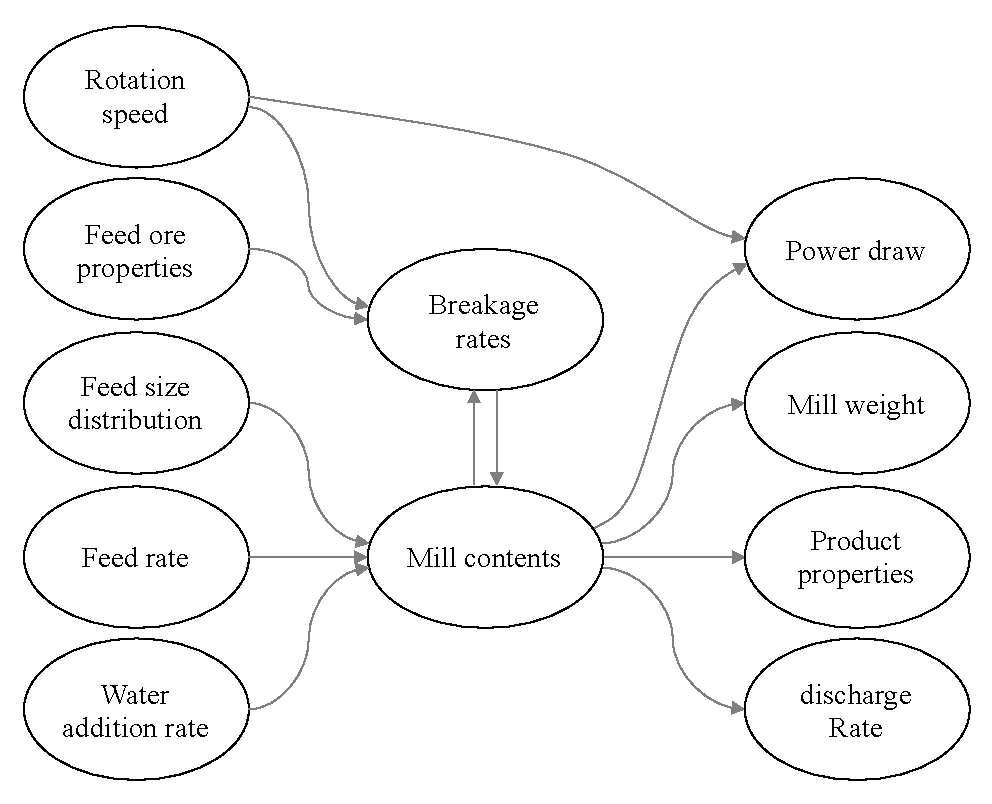
\includegraphics[width=11cm]{images/cause-effect.pdf}
	\caption{Cause and effect diagram} \label{fig:cause-effect}
\end{figure}

\cite{powell_applying_2009} highlighted the interactive (i.e. bi-directional) relationship between mill load and breakage rates and describe how these variables evolve dynamically. A change in ore feed properties, such as a change in hardness or particle sizes, leads to changes in the mill contents, which then affect breakage rates, which have a feedback effect on the evolution of the mill contents. This results in a non-linear response of the output variables which depend on the mill contents.

SAG mills are usually installed in closed-circuit with a pump and a classifier. Oversize material that passed through the discharge grate of the mill but does not meet the specification of the classifier is returned to the mill, sometimes via a crusher. This feedback mechanism includes a transport delay which further complicates the dynamic response of the process variables to changes in the inputs.

\subsection{Grinding process control}

The objectives of process control in grinding applications are firstly, to maintain a steady operation and secondly, to optimize the process conditions to achieve maximum operational benefits, for example, maximizing throughput while meeting the product particle size specification \citep{wei_grinding_2009}. Inevitably, trade-offs must be made between competing output variables, such as throughput and product particle size, and between product particle size and power consumption. The focus of this research is to identify and develop methods that facilitate the first objective (i.e. steady operation) given a set of desired operating conditions.

According to a 2007 worldwide survey of grinding circuit operators \citep{wei_grinding_2009}, 63\% reported that the \textit{proportional integral derivative} (PID) control technique was used. \textit{Multivariable control} or \textit{expert systems} were used by 21\%. Less than 10\% reported using \textit{model predictive control} (MPC) or adaptive (self-tuning) control.

The three most commonly controlled variables are the product particle size, the slurry level in the sump, and the sump discharge slurry density. The mill load or filling level also requires some form of control since excursions above or below the normal range can lead to undesirable conditions such as \textit{mill overload} and \textit{freewheeling} \citep{mcclure_overload_2015}. If the load becomes too high, the mill may have to be stopped, resulting in lost production \citep{wei_grinding_2009}.

The main manipulatable variables used for control are the flow rate of water to the sump, the flow rate of water to the mill, the feed rate of solids to the mill, and the discharge flow rate of slurry from the sump. Many modern mills also have variable speed drives which allow controlled variation of the rotational speed. However, in the 2007 survey results, use of speed as a manipulatable variable was reported by less than 10\% of respondents.

There is a considerable amount of academic literature on the application of process control theory and methods to grinding, going back as far as the 1980s, e.g. \cite{herbst_optimal_1988}. A wide variety of techniques have been proposed and evaluated since then. Most of the results are based on computer simulations of control systems applied to simulation models of grinding processes. In many cases, these simulations include ore disturbances.

\cite{najim_adaptive_1995} simulated various adaptive controllers applied to a grinding circuit model with a step disturbance in the ore hardness, represented by a -20\% reduction in breakage rates. The controllers regulate the circulating load and product fineness by manipulating the water addition rate and the fresh ore feed rate.

\cite{pomerleau_survey_2000} simulated various control algorithms applied to a grinding process consisting of a rod mill and a ball mill. The controllers manipulate the fresh ore and the water feed rates to regulate the product fineness and the circulating load. To compare the performance of the controllers, they simulate a sequence of disturbances to two ore properties---\textit{grindability} and feed size---as well as a change in the number of active cyclones, and set-point changes to control variables.

\cite{chen_disturbance_2009} propose a \textit{disturbance observer based} (DOB) control strategy applied to a ball mill grinding circuit model and evaluate its effectiveness in suppressing the effects of a 10\% increase in ore hardness on the product fineness and circulating load.

\cite{olivier_dual_2012} simulate the application of particle filtering to the estimation of both model states and parameters (known as \textit{dual estimation}) of a simulated primary grinding circuit and compare this approach to a simultaneous estimation method. The particle filtering approach is selected because of the non-linearity of the grinding model. They test both approaches in closed loop with decentralized PI controllers.

\cite{estrada_hybrid_2014} simulated a hybrid non-linear model predictive controller (HNMPC) to minimize specific energy consumption while regulating the product particle size. Hybrid approaches allow discrete variables to be included in the plant model. These are useful for representing processes which have discrete operating modes, such as those with equipment items that may be switched on or off during operation. They use this to represent changes in the stockpile feeding process and the activation of secondary grinding circuits and present simulation results showing how the controlled system responds as the different ore feed streams are switched off and on.

\cite{le_roux_throughput_2016} simulated a non-linear model-based control architecture to independently control the throughput and product quality of a grinding circuit. To achieve this, they use mill speed as a manipulatable variable, in addition to mill feed rate, water addition, and cyclone feed flow-rate. As in \cite{olivier_dual_2012}, the observer utilises a particle filter to estimate the mill states. However, their observer only utilises measurements that are commonly available in industrial plants, such as mill power and cyclone feed density.

\cite{botha_hybrid_2018} simulated a hybrid HNMPC for a primary grinding mill circuit in which the number of hydro-cyclones (a discrete variable) is used as an additional manipulated variable. The switching of hydrocyclones has a large dynamic influence on the plant. They show that this increased controller stability compared to a NMPC without this discrete variable.

\cite{aguila-camacho_control_2017} simulated various types of \textit{fractional order controllers} applied to a grinding circuit model with five manipulatable input variables (fresh ore feed rate, mill inlet feed water rate, sump feed water rate, cyclone feed flow rate, and ball addition rate) and three output variables (mill filling level, sump slurry volume, and product fineness). They also simulated step changes in the ore feed size distribution and in energy required to break ore particles, which is similar to ore hardness.

There is less literature available on the implementation, performance, and benefits of control systems in actual operations.

\cite{herbst_optimal_1988} presented results of implementing an optimal control algorithm (\textit{LQG control}) on a rod and ball mill grinding circuit in North America. This included use of an extended Kalman filter to estimate the states and parameters of a non-linear phenomenological model. The results show that the observer estimates tracked the process output measurements in response to a change in ore hardness, and the corresponding changes in model parameters.

\cite{hulbert_multivariable_1990} presented results of implementing a multi-variable controller on an AG mill in South Africa. The manipulated variables were feed rate of ore to the mill, feed rate of water to the sump, and flow rate of slurry to the cyclone. The control variables were product particle size, mill load, and slurry level in the sump. The results show the responses of the controlled system to set-point changes. They state that implementation of the multivariable controller resulted in better control of the product size and an increase in throughput.

\cite{desbiens_distributed_1997} describe the development and implemention of a PI-based regulatory control strategy on a grinding circuit at a mine in Qu\'ebec, including the steps of process model identification and filter design. The installed system regulates the pump box level, the cyclone feed density and the cyclone overflow density by manipulating the pump box water addition, the rod mill water addition, and the rod mill ore feed rate. 

One of the case studies presented in \cite{desbiens_using_2008} describes the implementation of an improved grinding circuit control strategy in a copper concentrator in Peru. The circuit consists of an open loop rod mill feeding three closed ball mill circuits via a flow splitter. In the prior situation, the position of the flow-splitter was adjusted by an operator, resulting in an uneven distribution of the rod-mill product among the ball mills. This had caused variability in the process outputs and sometimes overloading conditions in the ball mills. A second problem was the need to quickly adjust the rod-mill feed rate when a change in ore hardness occurred. The solution was to automatically manipulate the flow splitter and the rod mill feed rate according to the levels in the three pump boxes. After implementation of the new control system, the variability in process conditions reduced, the average throughput was increased by 4\%, and the combined circuit energy consumption reduced by 8\% to 10\%.

\cite{nunez_self-optimizing_2009} describe the development and implementation of regulatory controls at a mine in Canada. The grinding process consisted of two parallel circuits, each containing an open-circuit rod mill and a ball mill in closed-circuit. They reported that ore hardness changes were leading to either over or under-grinding and mill overload situations, which were not always detected in time by the operators. The new system consisted of two distributed control loops on each circuit, one to control the pump-box level by manipulating the rod mill feed set-point, and the second to control the cyclone overflow density (in the absence of a product particle size analyser) by manipulating the pump box water addition rate set-point. The results indicated a significant (60\%) reduction in variability of the product density and a 7.7\% increase in throughput for the same level of energy consumption, no change to mineral recovery, and the avoidance of mill overloads.

\cite{yutronic_sag_2011} describe the development and implementation of an MPC-based control strategy at a large concentrator plant in Chile. The primary goal was to reduce process variability in the SAG circuits, and in particular, the effects of poor sump level control on classification efficiency. The most important process variable was deemed to be the SAG filling level due to its relationship with grinding efficiency. Since filling level is not measurable, the mill weight was used as the control variable, along with the power draw, the shell impact noise level, the motor torque, and the produced pebble flow rate. The MPC included constraints on certain process variables, including the power draw to avoid electrical overload. The manipulatable variables were fresh ore feed rate, mill speed and the solids-to-water ratio of the feed. Two measured disturbances were also included in the MPC model, the returned pebble flow rate and the fine ore.

As a result of implementing the MPC system, the variability of the cyclone feed solids content and feed pressure were reduced by 43\% and 22\%, respectively. As well as reduced variation, other benefits were realised, including higher throughput, lower specific energy consumption, and a 4.8\% reduction in the average SAG product size.

C.W. Steyn, C. Sandrock (2013) present results of implementing MPC on an autogenous grinding (AG) mill in South Africa with the goal of reducing variability and to ``continuously drive towards the optimal operating point within system constraints.'' The two main control variables were power consumption and mill load. They report a 66\% reduction in power and a 40\% reduction in the standard deviation of the mill load as a result of implementing the MPC. This reduction in process variability also enabled steady-state experiments to be conducted to determine the optimal product particle size for a given mill feed rate, which lead to a subsequent improvement in mineral recovery.

\cite{gough_sag_2015} reports using MPC to control the mill weight, feed rate, and rotation speed of various SAG mills in mines in South America. The controller includes measured disturbances such as pebble recycle rate and ore size distribution as feed forward inputs to improve control. He presents results showing that the MPC is able to reduce the variability in mill weight (84\% reduction in standard deviation) and throughput (55\% reduction in standard deviation) compared to the expert systems that were used in these facilities, resulting in higher production rates.

\cite{bouchard_reducing_2017} showed how a properly designed control system can enable higher utilization of grinding circuit capacity and a reduction in specific energy consumption (kWh/ton). They used a simulation model of a rod and ball mill circuit to compare three different control strategies. Firstly, a typical basic regulatory (PI) strategy to control the pump box level by manipulating the water addition to the pump box and the hydro-cyclone pressure by manipulating the cyclone feed rate. Secondly, a regulatory (PI) strategy to control the pump box level by manipulating the rod mill feed rate, and the product particle size (P80) by manipulating the water addition to the pump box. Thirdly, an MPC (multi-variable) strategy to control the product size while maximising the rod mill feed rate, using all four manipulatable variables. The simulation results demonstrated that controlling the product size ensures not only that downstream process requirements are met and over-grinding is avoided, but can, in some instances, lead to higher throughput and hence, lower specific energy consumption.

\cite{liu_development_2018} analysed the mineralogical aspects of a grinding operation in Western Canada to determine the potential benefits of adjusting mill speed and load to offset changes in mill feed characteristics. However, the analysis is based on a steady-state simulation model and did not look at process control design aspects.

%% Although it mentions ore hardness changes, this is about ball mill process control.

%\cite{nunez_tecks_2019} describe a program of process control improvements on the secondary grinding process at a large copper concentrator in Canada.  The ore at this mine is sourced from three main pits and therefore exhibits high variability, including in hardness. While the primary grinding stage is the primary constraint from the perspective of maximising throughput, the objective of the secondary grinding control strategy was to adapt to feed changes to produce the smallest product particle size possible.
%
%The controlled variables were cyclone feed density and ball mill power consumption, and the manipulatable variables were pump box water addition rate and ball mill feed water addition rate. The improvements also included a real-time steel charge schedule, and the results show that the system reduced the product particle size from the grinding circuit by 7.5\%.

\subsection{Grinding process observers}

As mentioned above, one of the major obstacles to SAG process control and optimization is the lack of good online measurements (i.e. in real time) of critical process variables, in particular, breakage rates and the characteristics of the mill contents. Of the output variables shown on the right hand side of Figure \ref{fig:cause-effect}, only power draw is directly measurable. Mill weight may be inferred from load sensors or bearing pressure measurements. However, a reliable estimate of the weight of the mill contents is complicated by the fact that the total mill weight includes the weights of the shell and liners, which change over time due to wear. Direct measurement of the properties of the discharge of a SAG mill is also impractical due to the properties of the material flow.  Other measurements can be affected by high frequency measurement errors (noise) and others, such as particle size measurements, rely on physical analysis systems which can take minutes to produce new estimates.

For these reasons, process observers which produce reliable online estimates of the unmeasurable variables are an important tool in grinding process control.  As described above, \cite{le_roux_throughput_2016} and others have demonstrated the application of process observers in grinding process control simulations.  

As well as state estimation, it may also be necessary to identify model parameters online from measurement data, since these can be time-varying. \cite{le_roux_state_2016} investigated the state and parameter identifiability of a non-linear SAG mill model which included an explicit representation of the mill contents and breakage rates. They used six states to represent the volume of rocks, solids, coarse, fines, balls and water (the \textit{hold-up}) inside the mill. However, they found that measurements of the cyclone discharge flow rate and density were necessary for identifiability. Unfortunately, these measurements are not commonly installed in practice.

In \cite{le_roux_ekf_2017}, an extended Kalman filter (EKF) utilizing a simpler version of the mill model with three states (grinding media, solids, and water) to represent the mill contents is developed. They show that the states and parameters are linearly observable provided the mill discharge flow-rate, discharge density, and volumetric hold-up are measured. However, such instrumentation is also not available in industrial circuits because of space restrictions. They also note that measurements must be sufficiently accurate to reliably estimate the model states.

\subsection{Grinding process disturbances}

Continual variability in ore properties such as \textit{hardness}, \textit{competency}, \textit{particle size distribution} (PSD), and \textit{grade} (valuable mineral content) is normal in mining operations due to the geological characteristics of ore bodies. Additional variability is introduced by mining processes such as blasting and crushing, and during material handling operations such as shovelling, trucking, conveying, and storage. Storage systems such as stockpiles, for example, tend to cause segregation of material by particle size, which can result in dramatic changes in the particle size distribution of ore feeding primary grinding if the feed to the stockpile is interrupted \citep{estrada_hybrid_2014}. The nature of such variations will therefore reflect the particular processes and equipment employed at each site. Although they are not random, the complexities of these numerous effects is such that predicting the variations in the properties of ore arriving at the processing plant is extremely difficult.

There is limited available data on actual ore variability in real operations, especially on the dynamic nature of these variations. This may be attributed to the lack of cost-effective measurement technology, the cost of sampling and analysing ore, as well as the commercial sensitivity of such data.

\cite{hahne_ore_2003} carried out tests of ore samples from different points in the production process at a mine in Sweden. The results are used to estimate the influence of feed ore characteristics on grinding performance using a simulation model of the single stage autonomous grinding (AG) circuit. The simulations indicate that the net throughput with a coarse and hard ore is 10\% higher compared to fine and soft ore and that the fine–soft feed results in a coarser particle size distribution of the mill discharge. The amount of coarse material in the feed was found to be the most influential factor. They also found evidence that self-breakage occurs between the mine and the mill since the ore hardness (i.e. its resistance to breakage) increased with the distance from the mining face.

\cite{liu_development_2018} tested samples of different ores from a copper mine in Western Canada as part of a study of the potential benefits of variable speed drives for ball mills. He found that hardness, determined by standard \textit{Bond ball mill work index} tests, ranged from 20.2 kWh/t to 27.5 kWh/t. Both these values are in the category `very hard' according to Bueno, et al. (2015). The ore competency, which indicates its resistance to impact breakage, was determined using the JK drop weight test procedure and is expressed in terms of the $A\times{b}$ parameter (Napier-Munn et al., 1996). These were found to range from 29.2 to 39.7, which are categorized as `very hard' and `moderately hard'.

A mineralogical simulation model of the grinding circuits was used to estimate the theoretical maximum possible throughput for each ore type while achieving the desired product specification. They found that the achievable throughput with the least competent ore was 4 times higher than that of the most competent. This illustrates the severe impact that ore properties can have on a grinding operation. However, in the actual operation, different ores are blended to reduce the variation in operating conditions. Liu also estimated the optimal mill speeds to process each ore and found that these ranged from 57.2\% to 64.9\% of critical speed. At these speeds, mill power consumption ranged from 7306 to 9511 kilowatts (a variation of -11\% to +15\% of the average). These results provide a rare insight into the relationship between two important ore properties and grinding process conditions. However, it is unclear how generalisable these results are to other operations.

\textbf{TODO: Mention recent innovations in ore hardness testing and add a reference to HIT test studies done by \cite{kojovic_value_2019} (Agnico Eagle) and maybe include range of variation in hardness measurements measured.}


\section{Literature review – disturbance modelling}

%Outline notes:
%\begin{itemize}
%	\item Definition of a disturbance — unmanipulatable inputs to process.
%	\item Measured v. unmeasured (and unpredictable)— measured disturbances can be incorporated in a feed-forward control.  Unmeasured disturbances must be estimated in order to reject them.
%	\item TODO: Importance of considering disturbances in control system design.
%	\item Disturbance models and process observers.
%	\item \textbf{Should this section go in Method chapter?}
%	\item Two categories of disturbances: Infrequent, always-present.
%	\item Infrequent disturbances could have significant impact on process and control systems (MacGregor et al).
%	\item Standard approaches to system identification do not consider infrequent disturbances (focus on second order properties)
%	\item Need for broader range of disturbance model types and ways to incorporate them in control strategies.
%\end{itemize}

Few examples of academic work on characterising and modelling realistic industrial disturbances were found in the literature. Most of the literature on `disturbance models' or `disturbance characterisation' deals with the design of standard stochastic disturbance models, for example \cite{muske_disturbance_2002}, and \cite{pannocchia_robust_2003}, or is focussed mainly on detection and diagnosis of faults (i.e. unexpected disturbances), see \cite{thornhill_advances_2007} for example. In fault or anomaly detection, models of the normal behaviour of the process are used to identify when an \textit{unmodelled} disturbance occurs. Therefore, a typical fault detection algorithm does not have a model of the actual disturbance and its execution is suspended once the disturbance occurs and until normal operation has resumed. In contrast, the goal of this work is to use disturbance models for state estimation in the presence of disturbances.

Notable exceptions are some works on disturbances in specific applications such as wind power generation, vehicle suspension systems, and ship movement control. For example, \cite{papaefthymiou_mcmc_2008} used a Markov-chain Monte Carlo (MCMC) method to simulate wind speed for realistic dynamic simulations of renewable energy generation systems. An interesting stochastic process model, known as the \textit{bounded random walk process} (BRW), was found in the literature on economic modelling \citep{nicolau_stationary_2002}. This is used to represent economic or financial variables that have upper and lower limits, such as interest rates. Industrial processes variables also commonly have a normal operating range with lower and upper limits that are not exceeded during normal operation.

Nevertheless, a small number of research works are explicitly concerned with `realistic disturbances' (loosely defined) in continuous industrial processes. These are sometimes referred to as \textit{deterministic disturbances} to distinguish them from standard disturbance models based on stochastic noise models. One type of model in this category, which has received considerable attention, is described in the next section.

\subsection{Randomly-occurring deterministic disturbances} \label{RODDs}

\cite{macgregor_duality_1984} introduced the concept of the \textit{randomly-occurring deterministic disturbance} (RODD). This is a family of stochastic processes useful for modelling deterministic disturbances commonly encountered in real industrial processes, including  infrequently-occurring step changes, exponential changes, and ramps with changing slope. Disturbances of these types might result, for example, from set-point changes made by an operator or, relevant to this work, changes in the properties of material feeding a process. While these disturbances may be deterministic, the key issue is that they are not predictable by the control system. Therefore, representing them with a stochastic process driven by a random variable is a reasonable way to emulate the behaviour for the purposes of control system design.

The structural form of a RODD model is an \textit{autoregressive integrated moving average} (ARIMA) process fed by a special \textit{random shock} signal which has the value zero most of the time but occasionally, according to a defined probability, has a value sampled from a normal distribution. Depending on the choice of ARIMA process model, this can be used to simulate the different types of RODDs which may act on a process. The details of the RODD model are described in section \ref{subsec-RODD}.

MacGregor and coworkers also showed that the optimal control law derived for a process perturbed by a RODD is no different than that which would be derived for a process subject to a standard stochastic noise.  This is due to the common ARIMA structure of the models and the fact that the expected value (i.e. mean) of the random shock signal in the RODD model is zero as it is for a Gaussian noise. As a result, it is well-suited to process control design. For this reason, as well as its simplicity, the RODD model became a focus of this research.

\subsection{Detection and estimation of RODDs}\label{detection_RODDs}

\cite{robertson_detection_1995} described how unmeasured RODDs perturbing a system can be estimated online using a \textit{multi-model} observer approach. Traditional filtering methods such as Kalman filters are unable to efficiently estimate RODDs due to the inevitable trade-off that must be made between the ability to track the disturbance when it occurs and the sensitivity to noise at other times.

Multi-model filtering approaches involve simultaneously computing multiple independent filters with different parameters and then combining the estimates from these filters to produce a better estimate of the system states \citep{jaffer_estimation_1971, buxbaum_recursive_1970, tugnait_detection_1982}.

Since the sequence of past random shocks is not known, each filter's state estimate is calculated assuming a different hypothetical sequence of past shocks. The estimates of some filters are therefore better than those of others, depending on how closely the shock indicator sequences match the disturbances that actually occurred. The overall best estimate of the states is computed by calculating the conditional probabilities of each indicator sequence given the available measurement data, and this estimate is updated recursively each sample period using Bayesian inference.

Due to practical limitations, the optimal multi-model approach cannot be used in practice. Some kind of approximate method is needed to limit the number of filters required. Practical multi-model observers are therefore referred to as \textit{sub-optimal}.

Robertson and co. make use of three distinct approximations in their RODD observer design. Firstly, they define \textit{detection intervals} of more than one sample period and assume that the exact timing of a random shock is not important. This is based on the observation that when the correction gain of a Kalman filter is increased, it tends to remain large for several sample periods. Secondly, they rely on the fact that the random shocks are expected to occur infrequently, and thus, more than two (or some low number) of shocks are very unlikely to occur in the same detection interval. This further reduces the number of filters required, especially in systems subject to multiple independent RODDs.

The third approximation is referred to as \textit{sequence fusion}, which is also used in the \textit{generalized pseudo-Bayes algorithm} (GPB) \citep{jaffer_estimation_1971, buxbaum_recursive_1970, tugnait_detection_1982}. This is based on the assumption that only recent shocks have a significant affect on the estimates. Therefore, the length of the unique sequences which must be maintained is limited to a fixed number of sample periods, or detection periods.

Robertson and co. present results of simulating this sub-optimal multi-model observer on a 2-input, 2-output, non-linear dynamical system representing a continuous stirred-tank reactor (CSTR) process. They compare the estimates produced by the multi-model observer with two single extended Kalman filters (EKF) each with a different noise parameter. One of the EKFs is very sensitive to the measurement noise and the other is slow to respond to the RODD step disturbances, while the multiple-model observer performs better than either EKF in the example simulations.

\cite{eriksson_classification_1996} highlight the important differences between \textit{infrequent disturbances}, such as those produced by the RODD model, and \textit{omnipresent} disturbances. They argue that the standard stochastic noise model used in traditional system identification methods is unlikely to capture the effects of infrequent disturbances, despite the significant effect they have on the process. As a solution, they propose using a multi-model observer to simultaneously estimate and distinguish between different types of load disturbances. As an example, they demonstrate how this could be used to determine if a disturbance is acting at the input or the output of a process, given a batch of measurement data collected under closed-loop conditions.

This method involves grouping the filters of two (or more) multi-model observers into one combined multi-model observer. Each `bank' of filters represents a set of hypotheses relating to one of the possible disturbance models. The combined observer is then simulated on the data (offline) and the decision on which disturbance type is present is made based on which group of filters the most likely hypothesis belongs to. They provide results from simulation and a laboratory experiment to show that the method detects and estimates the actual disturbance in each case.

For the multi-model observer, they use an adaptive sub-optimal approach known as the \textit{adaptive forgetting through multiple models} (AFMM) algorithm by \cite{andersson_adaptive_1985}, also previously described by \cite{gustafsson_estimation_1993}. The AFMM algorithm employs a technique called \textit{sequence pruning} \citep{tugnait_detection_1982}, which is an alternative to the fixed-length \textit{sequence fusion} approach used by \cite{robertson_detection_1995} and \textit{hypothesis merging} techniques \citep{blom_interacting_1988}. Sequence pruning involves the online deletion of hypotheses that have a low probability given the current measurements. The deleted sequences are replaced by new sequences to represent only the possible branches of the most likely sequence at the next sample time. Thus, the total number of sequences and corresponding filters that need to be maintained remains constant. The AFMM algorithm also includes a procedure for online estimation of the measurement noise covariance, using a forgetting factor to control the speed of adaptation of the estimate \citep{andersson_adaptive_1985}.

In both multi-model observer approaches by \cite{eriksson_classification_1996} and \cite{robertson_detection_1995}, the process model and the magnitude and frequency of the actual disturbance are assumed to be known.

Robertson and Lee published a second paper a few years later \citep{robertson_method_1998}. In this paper they reference \cite{andersson_adaptive_1985} on the topic of multiple-model algorithms.  However, the approach and sub-optimal method used is very similar to that in their 1995 paper, except that a modification was made to the random shock variance parameter, which is applied at every update during the detection period rather than once. They also use slightly different terminology, dropping the term randomly-occurring deterministic disturbances in favour of \textit{infrequently-occurring abrupt disturbances}.

Simulation results using a different system are presented, a three-state non-linear model of a heptane to toluene aromatization process, along with sum-of-squared estimation errors, averaged over 50 different simulations, which makes it easier to compare the observer performance. The results show that their sub-optimal observer approach does 35\% better than either a single EKF or the standard GPB algorithm. This is attributed to the fact that their observer has a horizon of 90 minutes (using 22 filters), whereas the standard GPB algorithm has a horizon of only 2 minutes (using 16 filters), which is not enough to detect the shock occurrences.

\subsection{Disturbance modelling using hidden Markov models}
\label{hidden_markov_models}

\cite{wong_disturbance_2007} proposed a more general framework for modelling realistic industrial disturbances which have both continuous and discrete (i.e. modal) dynamics. In this framework, mode transitions are described by a finite-state \textit{Markov chain}. The model generating the Markov chain is referred to as a \textit{hidden Markov model} (HMM) because it has unknown parameters (transition probabilities) which must be inferred from available measurements. The combined system, including discrete and continuous dynamics is termed a \textit{Markov jump linear system} (MJLS) \citep{costa_discrete-time_2005}. The RODD model is a special cases of the MJLS.

%and other methods assuming noise inputs described by a \textit{mixture-of-Gaussians} (MOG),%

The HMM disturbance model can represent a much wider set of disturbances with complex switching behaviour, such as intermittent drifts, outliers, and white noise that is probabilistically interspersed with integrating white noise, which is an example of dual-regime behaviour. Although HMMs and MJLS's were not novel concepts at the time, the authors claim that their use for disturbance modelling prior to 2007 was limited. For references on prior work on MJLSs by the control community, they refer readers to \cite{costa_discrete-time_2005}.

Unlike \cite{robertson_detection_1995} and \cite{eriksson_classification_1996}, who focused on state estimation, Wong and Lee consider methods to identify the disturbance model from measurement data. The plant and Markov model parameters may be simultaneously estimated using \textit{maximum likelihood estimation} (MLE) methods, specifically, the \textit{expectation maximization} (EM) algorithm \citep{dempster_maximum_1977}.

For state estimation, Wong and Lee use a second-order generalized pseudo-Bayesian algorithm (GPB2)  \citep{bar-shalom_estimation_1993}. They present two numerical examples, comparing the prediction errors of the GPB2 observer using the identified MJLS model, averaged over 500 simulations, to those of the best observer with a stationary (i.e. non-switching) model, and to those of a GPB2 observer which uses the actual system model.  The results show that the prediction errors of the GPB2 observer with the identified model were only 6 or 7\% higher than those of the GPB2 observer with the true model, and both are significantly less than those of the stationary observer.

One important limitation of the HMM approach, which the authors note, is that it is difficult to determine whether a given MJLS is identifiable from input-output data \citep{vidal_observability_2002}. For this reason, they chose examples which only have switching in the noise parameters. Another problem is that MLE optimization is typically non-convex and the EM algorithm will usually only find local optima. To achieve the results presented, Wong and Lee chose initial settings for the unknown parameters that were known to be close to the optimum.

\cite{wong_realistic_2009} builds on the 2007 paper by demonstrating how the proposed HMM-based disturbance framework can be integrated into existing model-based control formulations. After introducing the HMM framework again, they present three simulated process control examples. The first demonstrates the use of the HMM disturbance framework for offset-free linear MPC on a single-input, single-output system. Multiple simulation scenarios with different combinations of high or low noise at the inputs and outputs are tested and one with switching noise levels. The results show that the proposed MPC designed with the HMM model and GPB2 estimator yields the best performance over all simulation scenarios, even when there is model-plant mismatch.

The second example demonstrates the closed-loop performance of the HMM control strategy in detecting and rejecting deterministic step changes. The controller is compared to a well-tuned controller with an integrated white noise disturbance model.

In the third example, the HMM framework is used to mitigate the impact of large variations in the concentration of the feed stream entering a nonlinear ethanol fermentation process simulation model. The concentrations of the feed are modelled as switching infrequently among several mean levels (low, mid and high) with the transitions governed by a Markov chain. In this example, a \textit{sequentially-linearized MPC} \citep{lee_extended_1994} is used and the effects of different types of feedback are compared---full state feedback including the Markov decision variable, Markov decision variable and output feedback only, and output feedback only.

Due to the difficulties of MJLS model identification mentioned above, they bypass the issue in this paper by assuming that the system, noise, and Markov parameters are known. Nevertheless, the authors concluded that the benefits of an HMM-based disturbance framework are ``most immediately'' gained by incorporating them within an existing control methodology such as MPC.

\subsection{Hybrid dynamical systems}

The \textit{hybrid dynamical system} is the most general definition, encompassing all dynamical systems which include both real-time (i.e. continuous) dynamics and discrete events \citep{van_der_schaft_introduction_2000}. As well as HMM-based models, it includes models with any other type of switching behaviour, such as those governed by logic.

Many physical systems and processes exhibit discontinuous behaviour (i.e. non-smooth changes in states such as steps or ‘jumps’). Since they are ubiquitous in nature as well as in human-engineered systems, the topic has received considerable attention in recent decades \citep{sworder_boyd_1999, bemporad_identification_2001, costa_discrete-time_2005, camacho_model_2010, djemai_hybrid_2014, estrada_hybrid_2014, guo_moving_2013, botha_hybrid_2018, bemporad_fitting_2018, oliveira_iterative_2020, piga_estimation_2020}. Methods of modelling and estimating hybrid systems could be applied to industrial disturbances, which are as multifarious and complex as other systems of interest in this research field.

\subsection{Non-linear system identification}

Since the types of disturbance models of interest in industrial process control are non-linear, or utilise non-Gaussian probability density functions, standard linear system identification techniques are not applicable. The literature on non-linear system identification is extensive and covers a wide variety of classes of non-linear systems \citep{schoukens_nonlinear_2019}. Indeed, the field extends well beyond control systems applications.

% TODO:
% Mention  signal processing, edge or step detection methods. Wavelets, TVR.

The central problem when a random variable input to a system is non-Gaussian, or when the system is non-linear, is that the posterior probability density distribution of the state and output variables may be non-Gaussian. In a discrete dynamical system, where the states are computed recursively over many time-steps, the analytical derivation of the posterior distribution at time $t$ becomes intractable, except in a few trivial cases (need reference).

Therefore, most approaches to non-linear system identification tend to be numerical in nature and involve approximations of the true (unknown) probability distributions. The \textit{Gaussian mixture model} (GMM) is one general technique used to represent diverse probability distributions (need ref).

% Note relevant:
% The task is more difficult because there are innumerable possible non-linear model structures, whereas in linear system identification, there is a finite and usually moderate number of model structures from which to choose.



TODO:
\begin{itemize}
	\item Briefly explain the emergent use of numerical methods such as sequential Monte-Carlo for non-linear system identification \citep{schon_sequential_2015}, which includes particle filtering (Arulampalam, 2002 tutorial)
	\item difference compared to MLE/EM (\textit{Marginalization} vs. \textit{Data augmentation} – simultaneous state and parameter estimation) and (\text{frequentist} vs. \text{Bayesian} methods).
	\item See overview diagram of methods in special issue of IEEE control magazine for an overview and cite this. \citep{wigren_nonlinear_2022}
	\item Variational inference \citep{ma_multiple-model_2019}.
\end{itemize}

\section{Objectives and contributions of this research}

The specific objectives of this research are:

\begin{enumerate}
	\item Propose a model for representing disturbances in grinding process operations
	\item Propose an observer framework using this model.
\end{enumerate}

% More specific objective?
%This work aims to address the problem of detecting and estimating infrequent, abrupt changes in the ore feed.

The main contributions of this research are:

\begin{enumerate}
	\item Evaluation of the capabilities of two multi-model observer algorithms by numerical simulation.
	\item Evaluation of the performance of a multi-model observer applied to state estimation of a simulated grinding process with an ore feed disturbance.
	\item Evaluation of the benefits of the multi-model observer as part of a simulated control system applied to a multivariable grinding process with an ore feed disturbance.
	\item \textbf{T.b.d.: A case study of the application of a disturbance model identification technique to characterise disturbances using simulated disturbance data and data from a real industrial operation.}
\end{enumerate}

